\chapter{Results} \label{cap:resultados}


%%Nos parâmetros de previsão de consumo no ICT Unifesp, a função ReLu ganha destaque para utilização em neurônios nas camadas ocultas da rede neural, por ser simples e eficiente para a aplicação nos experimentos, visto que na fase feed-forward tem efeito parecido com a função identidade, e na fase feed-backward durante o reajuste dos pesos pelo otimizador, conforme ilustrado na Figura \ref{fig:ReLu}, sua derivada produz efeito degrau zerando valores negativos e sendo adequada na aplicação do domínio destes parâmetros, visto que todas as variáveis endógenas e exógenas utilizadas como parâmetros de predição, como por exemplo pressão atmosférica, vendas e consumo de dias anteriores, datas, entre outros, não possuem valores negativos. Já a função linear ganha destaque para aplicação no neurônio de saída que determina o consumo previsto para uma data no futuro, pois na fase feed-backward do reajuste dos pesos pelo algoritmo de treino backpropagation, a derivada da função linear se torna zero, fazendo com que o algoritmo de treino transforme apenas os pesos sinápticos dos parâmetros de entrada os pesos sinápticos dos neurônios nas camadas ocultas da rede, sem interferir no neurônio de saída.

This chapter describes the main experimental results obtained during this research. As described in Chapter 4, the experiments were conducted in two phases. However, we have chosen to present in this chapter only the main results obtained. The other results are available in the Annexes to this document. The first sections introduce the organization of the data, a brief analysis of the variables and the experimental protocol, respectively.

\section{Organization of the data set}
%\TODO{descrever, nessa seção, como os dados foram organizados em treino, validação e teste}

    The data collection procedure was carried out according to the methodology of Section \ref{subsec:coleta_endogenos} for endogenous data, and according to the steps of Section \ref{subsec:coleta_exógenos} the exogenous data were obtained.
    Both sets of data collected were structured according to the Table \ref{table:dataset_final}, containing a time interval of records, from April 12, 2017 (2017-04-12) for the first record to December 16, 2019 (2019-12-16) for the last record, totaling 514 records of meal consumption on school days.
    
    According to the methodology defined in Section \ref{subsec:fases_experimentais}, this data set with a total of 514 records has been duplicated to 2 distinct experimental phases, each with a specific organization of the data set. The data set of the first experimental phase was organized according to the Figure \ref{fig:case1_timeline}. This phase has the validation set exclusively contemplating the first semester of 2018, indicating that the first semester of 2018 could present a consumption and sales movement similar to the first semester of 2019, being the ideal one for tests involving only the first semester of the test set.

    \begin{figure}[htb]
        	\center{        		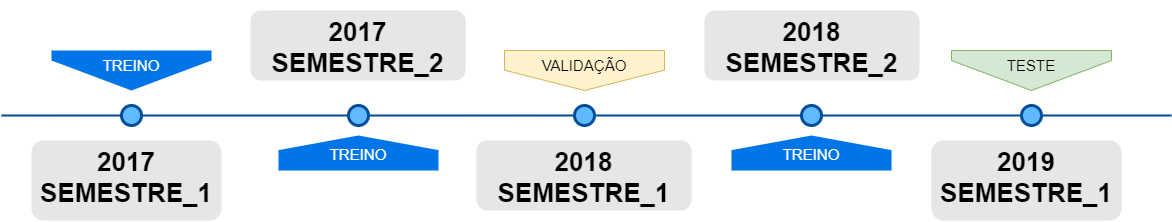
\includegraphics[width=1.0\textwidth]{./Figuras/resultados/case1_timeline.png}
        	 	\caption{Time domain of phase 1.} \label{fig:case1_timeline} }
        \end{figure}
    For the second phase the data set was organized according to the Figure \ref{fig:case2_timeline}. For this phase the selected validation set contemplated the entire school year of 2018, while for the model testing experiments the selected data contemplated the entire school year of 2019.
    
    \begin{figure}[H]
        	\center{        		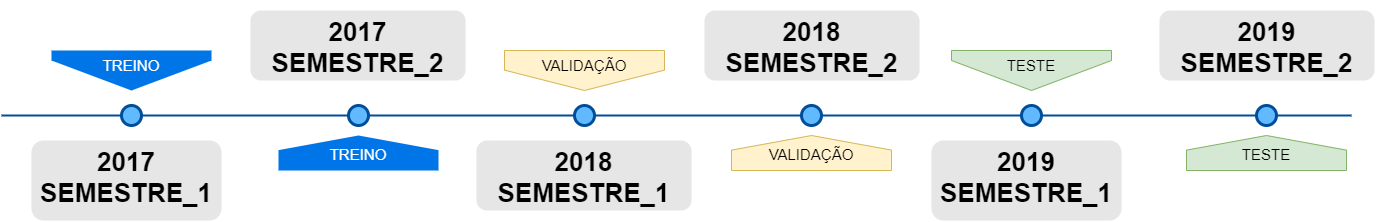
\includegraphics[width=1.0\textwidth]{./Figuras/resultados/case2/case2_dominio.png}
        	\caption{Time domain of phase 2} \label{fig:case2_timeline} }
        \end{figure}
   
    %\paragraph{Dificuldades encontradas e resolvidas}
    \subsection{Manipulation and pre-processing of the data set}
    
    Seeking to organize the raw data obtained for its subsequent application in the models, some peculiarities were found. The first difficulty found in the experiments was an anomalous behavior of the forecast results for model RNN\_ENDO\_2. The blue line in Figure \ref{fig:pandas_wrong_indexing} represents a meal forecast of model  RNN\_ENDO\_2, and the red line real consumption values of the first half of 2019. In this way, it was possible to observe that in both sets (real and predicted) this behavior was present. 
    
    \begin{figure}[!htpb]
    	\center{
    		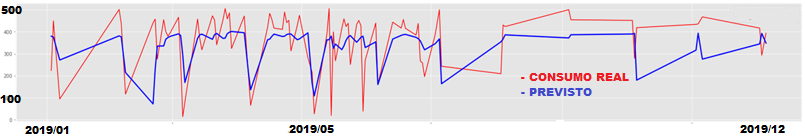
\includegraphics[width=1.0\textwidth]{./Figuras/resultados/pandas_wrong_indexing.png}
    	\caption{Result of  RNN\_ENDO\_2 model obtained on the data set randomly ordered over time.} \label{fig:pandas_wrong_indexing} }
    \end{figure}
    
    After an exploratory analysis it was discovered that the records contained an error in the indexing by date, where the date stamp was changed, that is, the days by months and vice versa. After the correction of this indexing problem the actual consumption and forecast data produced realistic results and within the expected format, as presented in Figure \ref{fig:pandas_correct_indexing},  that presents an example of prediction by model RNN\_ENDO\_2 and the real data for the lunch period.
    \begin{figure}[!htpb]
    	\center{
    		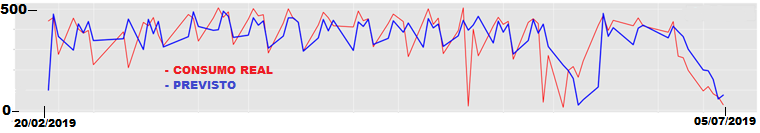
\includegraphics[width=1.0\textwidth]{./Figuras/resultados/pandas_correct_indexing.png}
    	\caption{Result of RNN\_ENDO\_2 model obtained on the data set with corrected order. } \label{fig:pandas_correct_indexing}}
    \end{figure}
              
\section{Variable Evaluation}
During this section some comments will be made about the variables characteristics that were most important to the problem, and some graphs will be presented from the statistical study done to evaluate the relationships among them. 

    \subsection{Refectory consumption estimates}
    
        The analysis of the estimation technique of consumption, performed subjectively in relation to the consumption of the previous week, uses the calculation of  30\% of production above the consumption of the fifth previous day. This estimation method is adopted to tolerate discards due to the existence of a contractual fine for lack of meals. Still, it is possible to observe that this model of  30\% more produces a linear behavior, represented by the blue line in the Figure  \ref{fig:ru_pred},  being distant from the real consumption behavior, indicated by the red line. 

        \begin{figure}[!htbp]                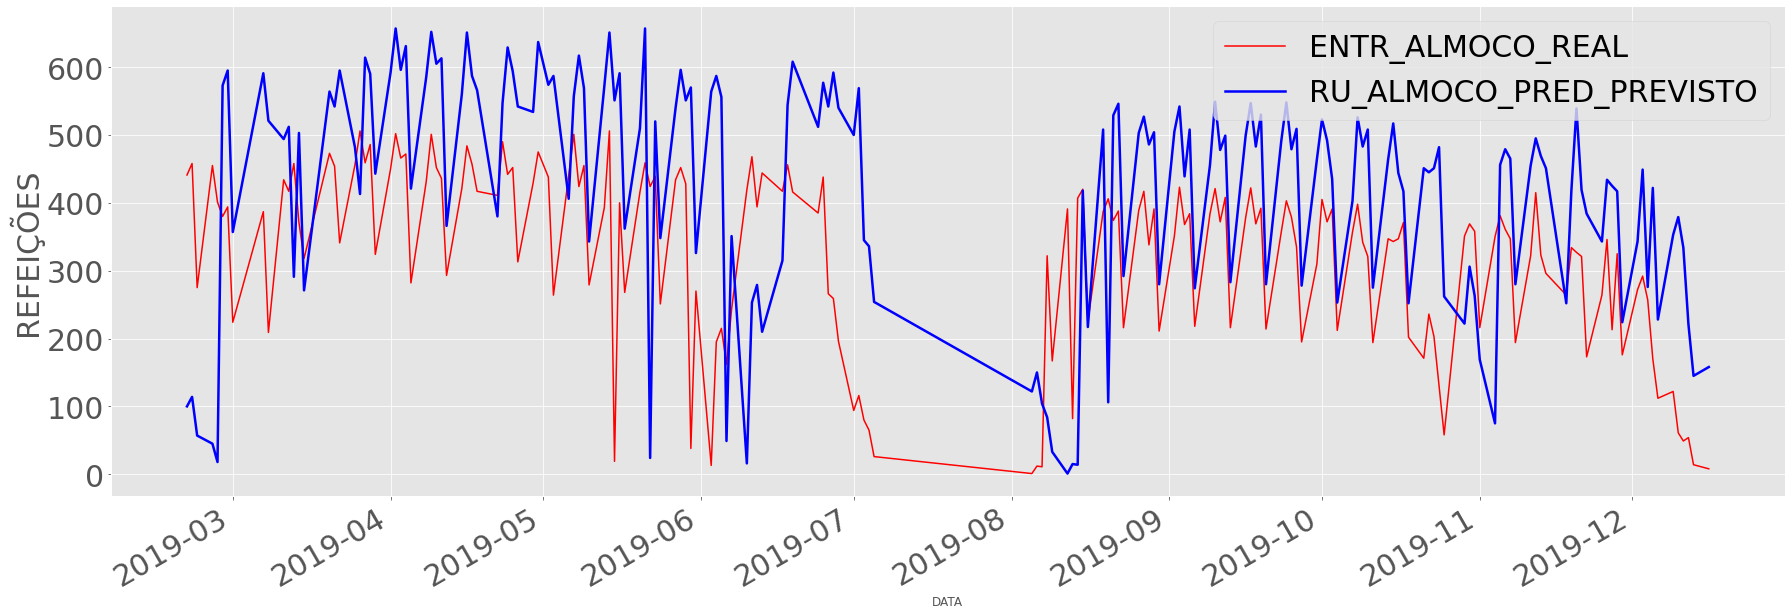
\includegraphics[width=\textwidth]{./Figuras/resultados/case1_ru_pred.png}
                \caption{Refectory estimate for 2019.} \label{fig:ru_pred} 
        \end{figure}

            
        
        Although the estimate follows the trends of falls and increases in consumption, the Figure \ref{fig:ru_pred_scatter} shows the dispersion generated between the estimate of the R.U and the actual consumption in the year 2019, showing that the linear regression (red line) has the axis totally decentralized with the function identity of the ideal estimate (represented by the imaginary diagonal formed between the origin of the graph and the top right vertex). 
        

                \begin{figure}[ht]
                    \center{                    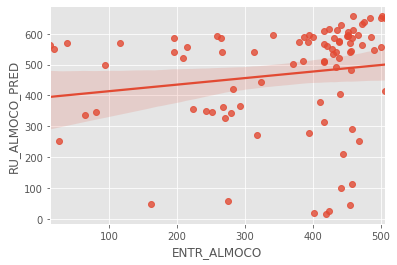
\includegraphics[width=0.6\textwidth]{./Figuras/resultados/case1_ru_pred_scatter.png}
                    \caption{Scatter plot of the refectory's estimated consumption for the year 2019.} \label{fig:ru_pred_scatter} }
                \end{figure} 

        
        
        Thus, this format of prediction also generates an error higher than 30\% in the total amount of meals discarded during the semester, caused by the oscillatory behavior of consumption, according to the table \ref{table:case2_rupred}.

            \begin{table}[!ht]
            \centering
            \rowcolors{2}{gray!25}{white}
                \begin{tabular}{c|c}
                \rowcolor{gray!50}
                \hline
                \multicolumn{2}{c}{Consumption with margin 30\% above the previous day 5}\\ \hline     
                TOTAL MEALS CONSUMED & 58653  \\
                TOTAL ESTIMATED MEALS & 76262 \\ 
                CORRELATION (r)&  0.4006 \\
                P-value & 2.0845e-08\\
                RMSE & 191.7620 \\
                SUM OF POSITIVE ERRORS & 23412 \\
               SUM OF NEGATIVE ERRORS  & -5803 \\
                AVERAGE ABSOLUTE ERROR & 133.0 \\
                ABSOLUTE ERROR AVERAGE PERCENTAGE & 205.6113\% \\  \hline 
                \end{tabular} \caption{Metrics of the refectory's estimated consumption for the year 2019}
            \label{table:case2_rupred}
            \end{table}

    \subsection{Analysis of endogenous variables}
    
        The endogenous variables are the input time parameters in the MLP and GRU models, corresponding to the consumption domain in the restaurant.
         % \newpage
        \subsubsection{Consumption of the current day in relation to the previous day's ticket sales}
        
        It is possible to notice in the Figure \ref{fig: case1_consumo_vendas_almoco} that ticket sales in the lunch period showed a different behavior in 2017 compared to the following years due to a limitation imposed by the refectory, from 2018 onwards students could purchase only 2 tickets per day. Possibly, this limitation was given to approximate the consumption behavior of 1 or 2 days after the ticket sale. This limitation can be interpreted as a management aid method for meal production and waste treatment.
        
        \begin{figure}[h]
                    	\center{                    		        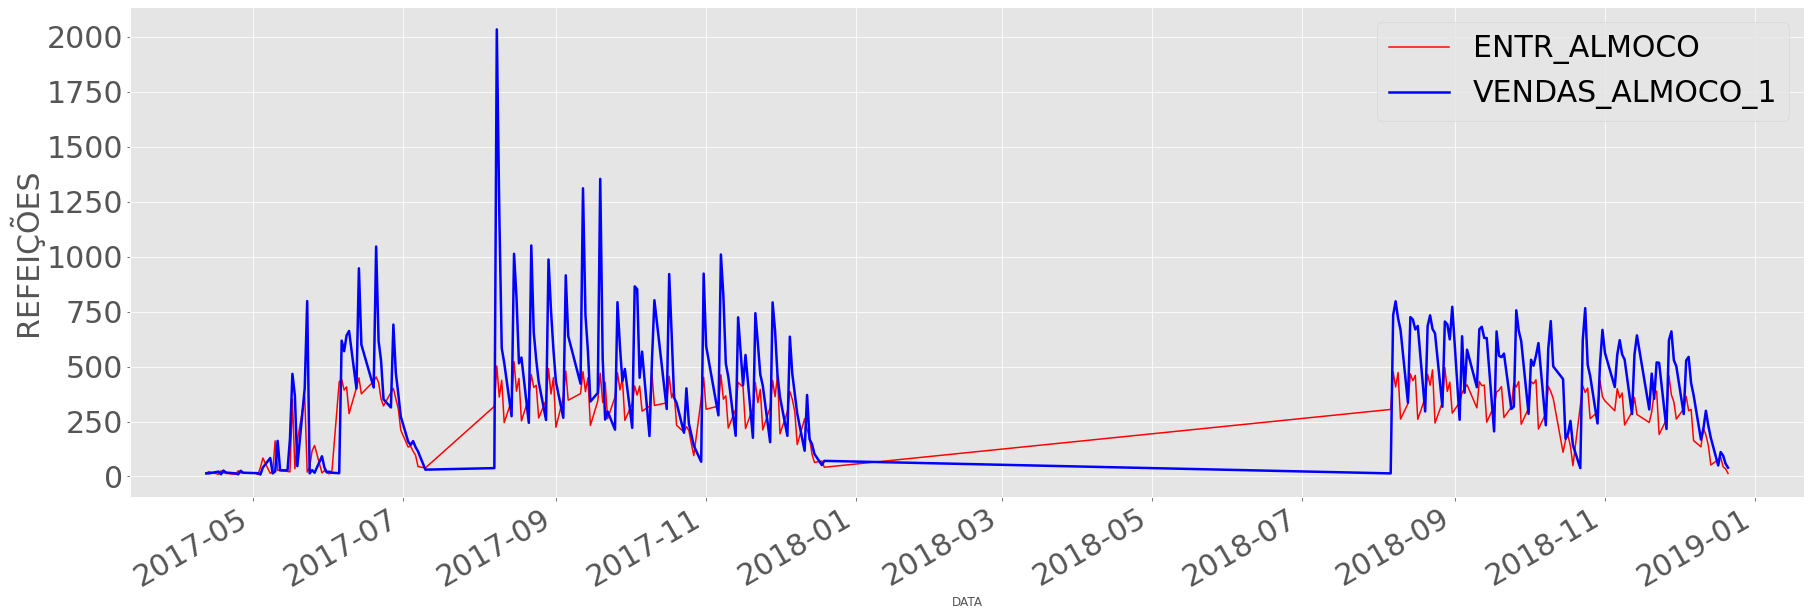
\includegraphics[width=0.8\textwidth]{./Figuras/resultados/case1_consumo_vendas_almoco.png}
                    	\caption{Correlation between consumption and lunch sales.} \label{fig: case1_consumo_vendas_almoco} 
                    	}
                    \end{figure}
	        
       Even with the \textit{outlier} value of 2000 sales in a single day, and with the new limitation on ticket purchases from 2018 onwards, consumption at lunchtime is strongly related to ticket sales in the previous day's lunch period. It is also noted that students have adapted to the limitation imposed for the use of tickets with a validity period of only two days, as the value of the correlation coefficient is approximately 72\%, as shown in the table \ref{table:case1_vendas1}.
        
 \begin{table}[!htpb]
           \centering
           \caption{Comparison of consumption with a previous day}
             \rowcolors{2}{gray!25}{white}
             \begin{tabular}{c|c}\hline
                \multicolumn{2}{c}{CONSUMPTION IN RELATION TO SALES OF 1 DAY BEFORE}\\ \hline
                CORRELATION (r) &  0.7255528038157009\\
                P-value &5.399561176138223e-41\\
                RMSE & 260.5399426736619\\
                AVERAGE ABSOLUTE ERROR & 139.0\\
                ABSOLUTE ERROR AVERAGE PERCENTAGE & 90.18\\\hline
            \end{tabular} \label{table:case1_vendas1} \end{table}
    	            

        
        There are other unscheduled factors involved, such as possible failure of sales records in the system, as well as the \textit{outlier} value of 2000 sales can be interpreted with the system and meal database migration that occurred in 2017 from the Talim unit of ICT-Unifesp to the Hospital São Paulo database. Possibly also sales were imported from the old system without the differentiation of dates.
        
        The total of meal sales at lunchtime was 242282 for all 514 entries in the data set. In this same period the actual consumption value, meaning students who effectively entered the refectory (passed through the turnstile) totaled 163752 meals. Although notorious, the difference of 78,530 meals sold above the actual consumption was not able to be investigated in this work. It should be noted that these figures were obtained from the original set of data provided by the ICT-Unifesp R.U contract inspector through an e-mail request to this inspector.


                    \begin{figure}[!htpb]
                    	\center{                    		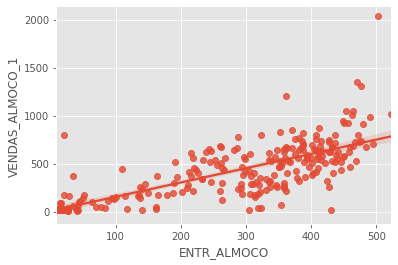
\includegraphics[width=0.7\textwidth]{./Figuras/resultados/case1_scatter_consumo_vendas_almoco.png}
                    	\caption{Dispersion graph between consumption and lunch sales.} \label{fig:case1_scatter_consumo_vendas_almoco} }
                    \end{figure}
                
                
          

            \subsubsection{Normalization and scale of \textit{features}}
            
                The process of normalization and scale is demonstrated in this Section with a \textit{feature} of sales of  \textit{tickets} from 1 previous day, because among all this is the one that has produced \textit{outliers} of greater prominence.
                The data normalization is done with the ceiling of 3x the average standard deviation, so the peak of 2000 sales was normalized to the rounded value of 1356 meals. Even with the normalization, the linear behavior of this \textit{feature} was maintained, as presented in the Figure \ref{fig:feature_sem_outliers}. 

                
                        \begin{figure}[H]
                        	\center{
                            	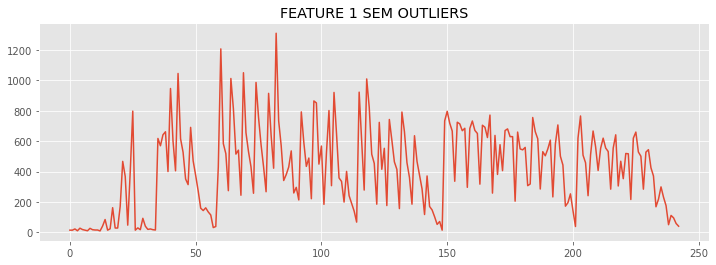
\includegraphics[width=0.9\textwidth]{./Figuras/resultados/feature_sem_outliers.png}
                            	\caption{Sales of normalized \textit{tickets} with 3x the standard deviation ceiling.}
                            	\label{fig:feature_sem_outliers}
                        	}
                        \end{figure}
                        
                        
                        After normalization, the scale was standardized from 0 to 1 in this one and as it is observed in Figure  \ref{fig:feature_sem_outliers_escalada}, the linear behavior was maintained again.
                        
                        \begin{figure}[H]
                        	\center
                        	{                    		
                            	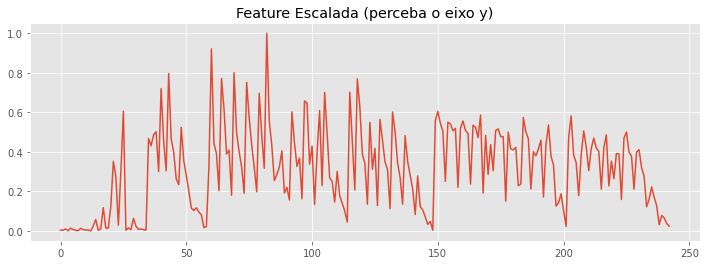
\includegraphics[width=0.9\textwidth]{./Figuras/resultados/feature_sem_outliers_escalada.png}
                            	\caption{Sales of \textit{tickets} climbing from 0 to 1.} \label{fig:feature_sem_outliers_escalada} 
                        	}
                        \end{figure}
                       
                This process of normalization and scale has been carried out for all endogenous metrics and also for climate metrics.
        	   % \newpage
        	   
                \subsubsection{The current consumption in relation to the previous day's dinner.}
                %\TODO{QUILES - esse foi um dos fenômenos mais curiosos que encontrei e que não tenho explicação pra ele, o consumo da turma da noite é muito parecido com o consumo da turma do almoço do dia seguinte}
                
                %\TODOR{Isso não foi erro de carregamento dos dados? caso esteja tudo certo, pode deixar assim. De qualquer forma, mencione isso no texto como um achado.}
                Looking to find and evaluate the possible relationship between the various metrics used, this analysis gained relevance as an anomalous and probably casual effect found among the data.
                Although the curricular schedules of students consuming meals at lunch are usually fired at students consuming dinner the night before, a clear relationship between these 2 variables can be detected.
                 This behavior can be evidenced by the congruence between the parameters, as shown in figure \ref{fig:case1_consumo_jantar} and by the high correlation obtained in the linear regression (R = 0,7655) between these 2 consumptions, presented in figure  \ref{fig:case1_consumo_jantar_scatter}. Even though it presents a relevant correlation, it was not possible to determine an evident cause for this anomalous effect found.

                
  
                \begin{figure}[H]
                	\center{
                	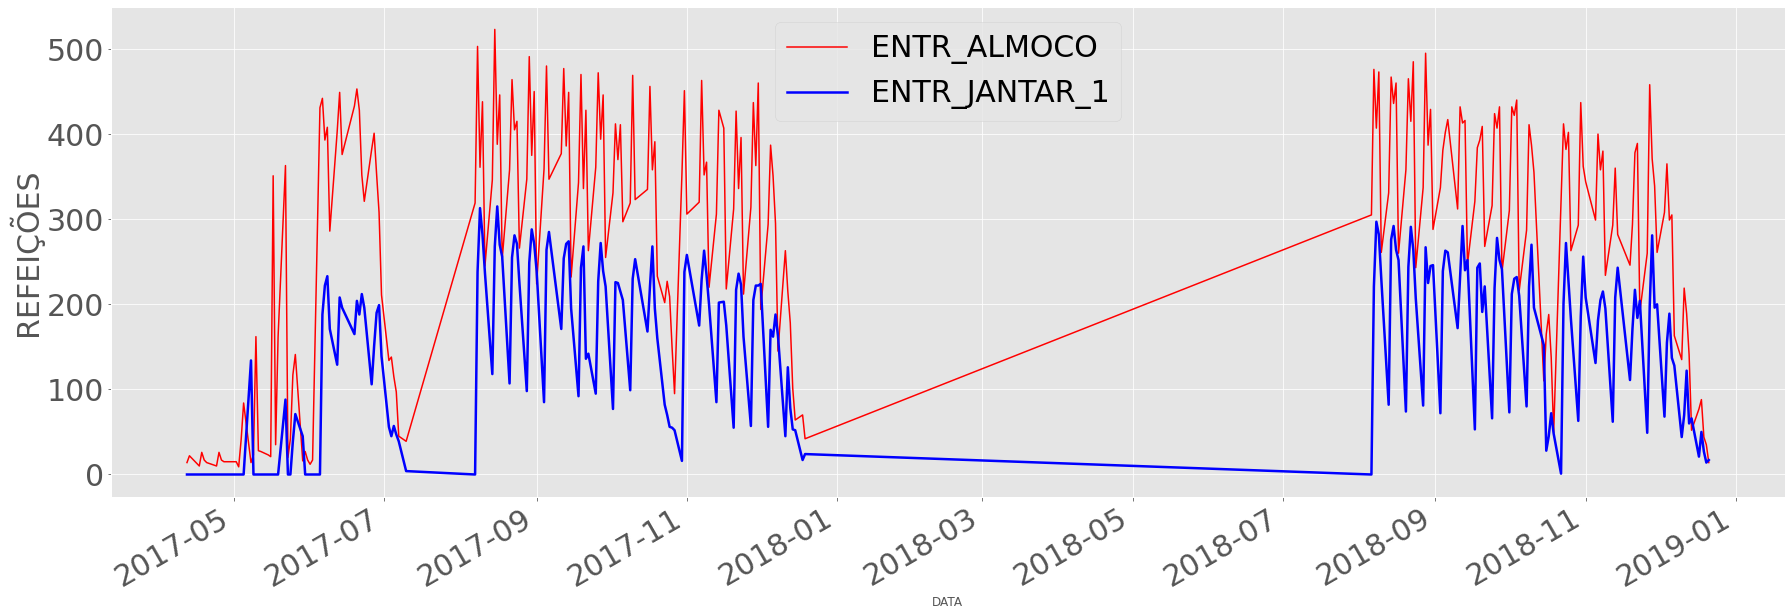
\includegraphics[width=0.8\textwidth]{./Figuras/resultados/case1_consumo_jantar.png}
                	\caption{Correlation of lunch and dinner consumption from 1 previous day.} 
                	\label{fig:case1_consumo_jantar} }
                \end{figure} 
               
                \begin{figure}[H]
                	\center{                    		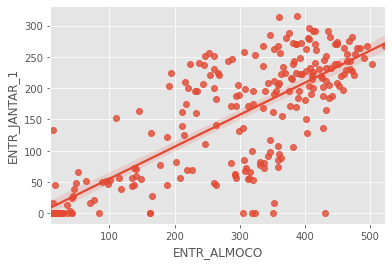
\includegraphics[width=0.8\textwidth]{./Figuras/resultados/case1_consumo_jantar_scatter.png}
                	\caption{Graph of dispersion between consumption and dinner of 1 previous day.} 
                	\label{fig:case1_consumo_jantar_scatter} }
                \end{figure}
             
            
    	    \subsection{Weekly Seasonality Analysis}
    	        The following consumption graphs from Figure 5 \ref{fig:case1_violinplot_segunda}, representing the Monday, up to figure \ref{fig:case1_violinplot_sexta}, representing Friday, are generated for the binary categorical \textit{features}, with the \textit{violin-plot} functionality in the library \textit{seaborn}, appropriate for distribution of binary categorical variables in a data set.
    	        
    	        The blue violin with the value 1 represents the distribution of consumption across the total data set.
    	        The violin with value zero can be ignored and is a standard return on the tool graph, representing the consumption complement for the day of the week considered.
    	        On Fridays, the consumption had a smaller distribution scale for the whole set 2019. It was noticeable that despite the alternation of time slots during the exchange of semesters in the year 2019, the days of Tuesday and Thursday concentrated the largest movement of consumption.
    	       %\newpage
    	      { \begin{center}    
    	        \begin{minipage}[c]{0.45\textwidth}
    	         \begin{figure}[H]
                	\center{                		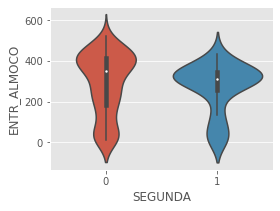
\includegraphics[width=\textwidth]{./Figuras/resultados/case1_segunda.png}
                	\caption{Gráfico de violino da distribuição do consumo na segunda feira.} \label{fig:case1_violinplot_segunda} }
                \end{figure}\end{minipage} \hfill %
                \begin{minipage}[c]{0.45\textwidth}
                \begin{figure}[H]
                	\center{                		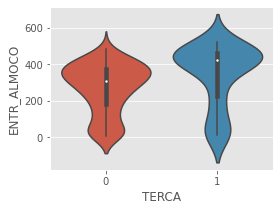
\includegraphics[width=\textwidth]{./Figuras/resultados/case1_terca.png}
                	\caption{Violin graph of Tuesday's consumption distribution.} \label{fig:case1_violinplot_terca} }
                \end{figure} \end{minipage}
                
            \begin{minipage}[c]{0.45\textwidth}
                \begin{figure}[H]
                	\center{                		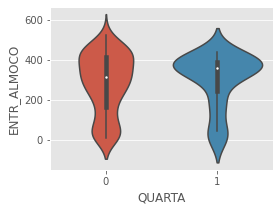
\includegraphics[width=\textwidth]{./Figuras/resultados/case1_quarta.png}
                	\caption{Violin graph of Wednesday's consumption distribution.} \label{fig:case1_violinplot_quarta} }
                \end{figure}\end{minipage} \hfill %
                \begin{minipage}[c]{0.45\textwidth}
                \begin{figure}[H]
                	\center{                		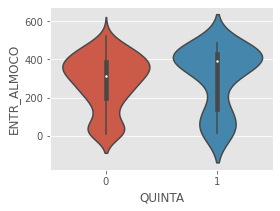
\includegraphics[width=\textwidth]{./Figuras/resultados/case1_quinta.png}
                	\caption{Violin graph of Thursday's  consumption distribution.} \label{fig:case1_violinplot_quinta} }
                \end{figure}\end{minipage} %
                        \begin{minipage}[c]{0.45\textwidth}
                \begin{figure}[H]
                	\center{                		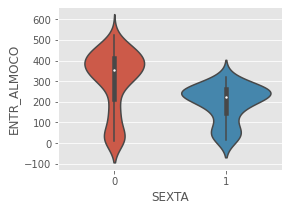
\includegraphics[width=\textwidth]{./Figuras/resultados/case1_sexta.png}
                	\caption{Violin graph of Friday's consumption distribution.} \label{fig:case1_violinplot_sexta} }
                \end{figure}
                \end{minipage} \end{center} }
    \subsection{Exogenous variables analysis}
        The exogenous variables correspond to the discrete domain parameters, which are used exclusively in mixed neural network models and are read by the MLP layers of these models.
        
        \subsubsection{The current consumption in relation to the advance of the semester.}
        
        For this analysis it was necessary to restrict the domain of analysis to 1 semester, the consumption in relation to the advance of the semester had an abrupt fall in the last days of the semester, and thus the correlation of the data sets of figures \ref{fig:case1_perc_sem} and \ref{fig:case1_perc_sem_scatter} obtained negative value.
        
                \begin{figure}[H]
                	\center{                    		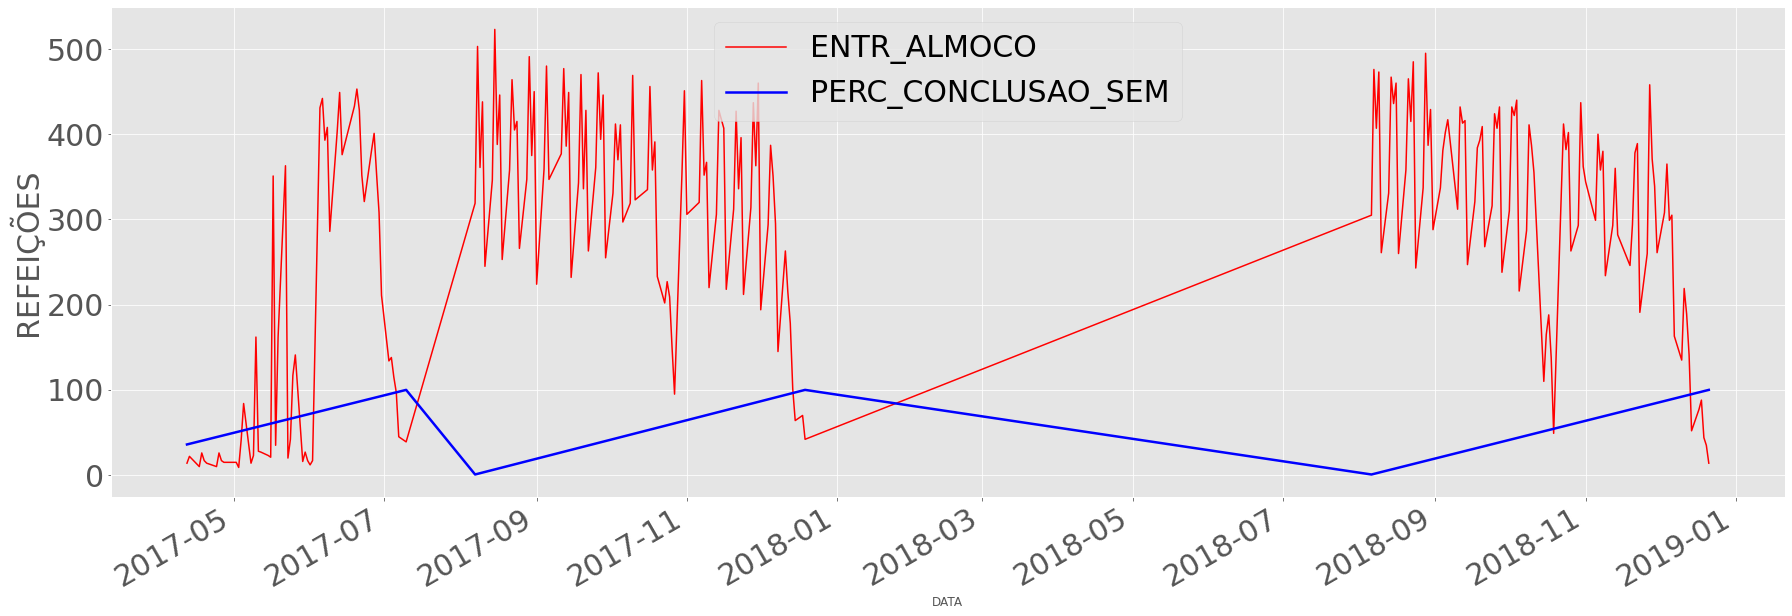
\includegraphics[width=\textwidth]{./Figuras/resultados/case1_perc_sem.png}
                	\caption{1st Phase : Relation between consumption distribution and semester's advance, Correlation (r) = -0.35.}
                	\label{fig:case1_perc_sem}
                	}
                \end{figure}  

        
                       \begin{figure}[H]
                	\center{                		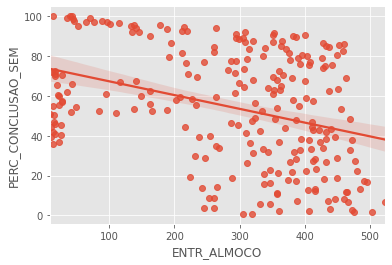
\includegraphics[width=\textwidth]{./Figuras/resultados/case1_perc_sem_scatter.png}
                	\caption{Graph of dispersion of consumption distribution as the semester progresses.} \label{fig:case1_perc_sem_scatter}
                	}
                \end{figure}
           

\section{Experimental Protocol}
%\TODO{faça um resumo sobre as duas fases e as principais diferenças entre elas. Na sequência, detalhe os detalhes do principal modelo obtido (o com melhor resultado de predição)}
    In this section will be started the experiments with the Neural Network models.
    The first experiment evaluates the learning potential of the models in predicting R.iU consumption, through a basic neural network model, by concluding that the most basic neural network topologies have learning potential about the problem.
    Then, the topology was selected and the experimental phase that brought the best results and finally it is analyzed and indicated as the final solution of the project.
    
    \subsection{Evaluation of the learning problem of meal prediction through MLP Neural Networks}
        \subsubsection{Empirical topology adjustment of the first perceptron model}
        
        The first neural net experiment performed in the first experimental phase evaluated the learning capacity of the perceptron model on the seasonality of endogenous data, referring to the domain of meal consumption in the R.U., verifying if the consumption behavior in the refectory could be learned by this type of neural net, therefore 1 initial perceptron net was defined with only 1 hidden layer containing 1 neuron for 15 input parameters (same number of endogenous parameters) and with 1 output neuron, called MLP1.
        
        The parameters endogenous correspond to an interval of 5 days prior to the consumption of meals in the lunch period, dinner and ticket sales in the lunch period.
        The model was named MLP1, its illustration can be seen in figure \ref{fig:case1_mlp1} obtained by using the NETRON tool.  
        
        \begin{figure}[H]
        \center{
        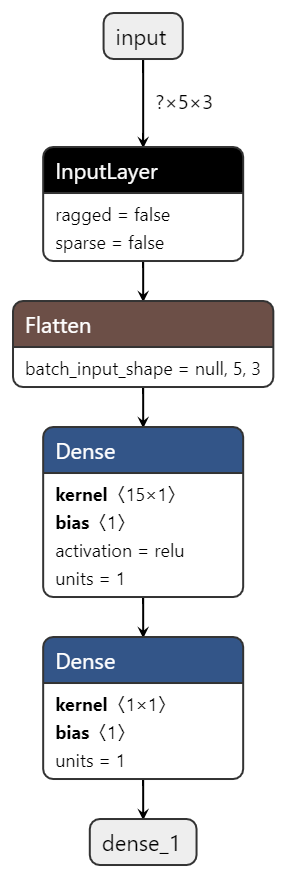
\includegraphics[width=0.3\textwidth]{./Figuras/resultados/case1_MLP1_validated.png}
        	\caption{Topology of MLP1 model, NETRON tool.} 
        	\label{fig:case1_mlp1}
        }
        \end{figure}
        
        
        Each layer of the MLP1 model corresponds to a block with title  \textbf{Dense}  in this Figure, the first edge of the figure between the \textit{input} and InputLayer shows the 3 time series of the input parameters, with an interval of 5 days each. \textbf{ENTR\_LUNCH, ENTR\_DINNER e SALES\_LUNCH}. The Flatten block converts each day of time series input into an MLP neural network input parameter, according to the conceptual model of the \citeonline{Lopes2008}work illustrated in figure  \ref{fig:mlp-lopes} which uses only 1 endogenous parameter with an interval of 5 days also. The first hidden layer of this network can be visualized in the first dense block of the figure that demonstrates the ReLu activation function of this neuron, and the number of units of this layer being 1.
        The output layer is the last block of the figure, also with 1 unit and since the activation function is linear, it is not displayed in the block description.

        
        The training of this model was executed obtaining RMSE with the value 130.62 over the validation set, in this case the first phase being the data of the first semester of 2018, and it is possible to notice in figure \ref{fig:case1_mlp1_train} that the lines of the loss and training function demonstrated an adequate training until the last training season, and as there was no application of simultaneous Validation Loss with Train Loss, the training did not produce an overfitting.
        \begin{figure}[H]
        	\center{
        	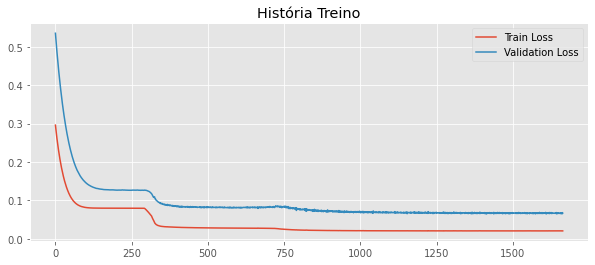
\includegraphics[width=0.8\textwidth]{./Figuras/resultados/case1_mlp1_train.png}
        	\caption{Model training graph MLP1, RMSE = 130,62}
        	\label{fig:case1_mlp1_train}
        	}
        \end{figure}
        
        Therefore, the depth of the MLP1 model was increased by obtaining the MLP2 model with topology illustrated in figure \ref{fig:case1_mlp2} and after training this model it was possible to notice the decrease of the RMSE to the value of 107.97, as observed in figure \ref{fig:case1_mlp2_train}. It is possible to realize that from the 300 training season on, the Train Loss line began to suffer a decrease in error as the Validation Loss began to gain error from the 400 season on. As the reconfiguration of the network topology produced improved results until an overfitting saturated this improvement for this topology, it was validated the hypothesis that the prediction of consumption in the refectory can be learned by simple models of Neural Networks, and therefore the research followed with the definition of new models demonstrated in the next section.
        \begin{figure}[H]
        	\center{
        		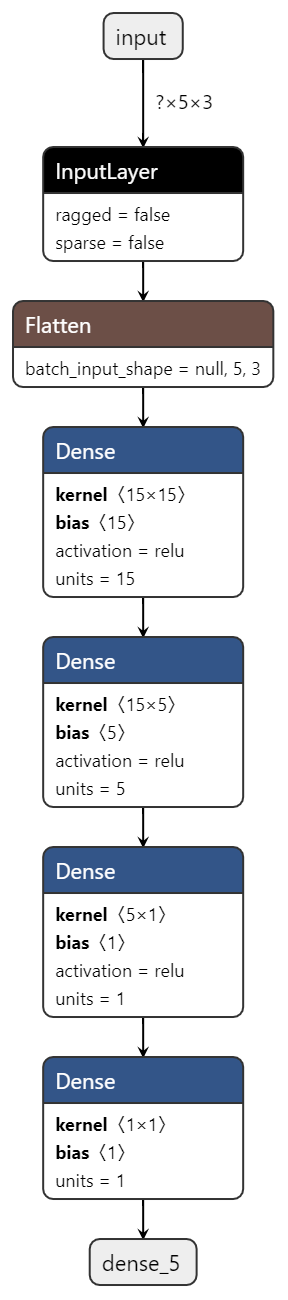
\includegraphics[width=0.3\textwidth]{./Figuras/resultados/case1_mlp2.png}
        	\caption{Model Topology MLP2.} \label{fig:case1_mlp2} }
        \end{figure}
        \begin{figure}[H]
        	\center{
        		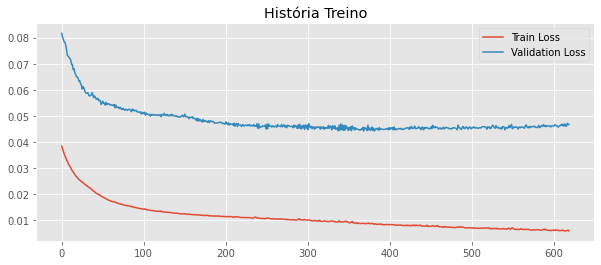
\includegraphics[width=1.0\textwidth]{./Figuras/resultados/case1_mlp2_train.png}
        	\caption{Model training graph MLP2. RMSE = 107,97.}
        	\label{fig:case1_mlp2_train} }
        \end{figure}
        
    \subsection{Topologies of best models}
    
    In this section some comments are made about the topologies of the models that obtained results presented with schematic figures of the network. For the rest of the trained models, the same procedure is done in annex \ref{cap:anexo1}.
         
        \subsubsection{Mixed Model RNN\_EXO\_1, best result in the second phase and in all the whole work}
            Interpreting the digram of the first mixed model, RNN\_EXO\_1, in figure \ref{fig:case1_rnn_exo_1} the block with the GRU title on the left in the topology figure of the model deals with endogenous (temporal) inputs, as exemplified in endogenous GRU models. The block with title \textbf{Dense} is an MLP network that receives a input with 10 parameters of 1 dimension, consequently all discrete, corresponding to the 4 climatic parameters (temperature, humidity, pressure and wind), 1 parameter for the current day of the week, 1 for the current semester and 4 calendar control parameters (distance from the previous date, later, semester advance, month advance). The output of the GRU and MLP blocks are concatenated and treated by the output MLP block.
            \begin{figure}[H]
              \center{
                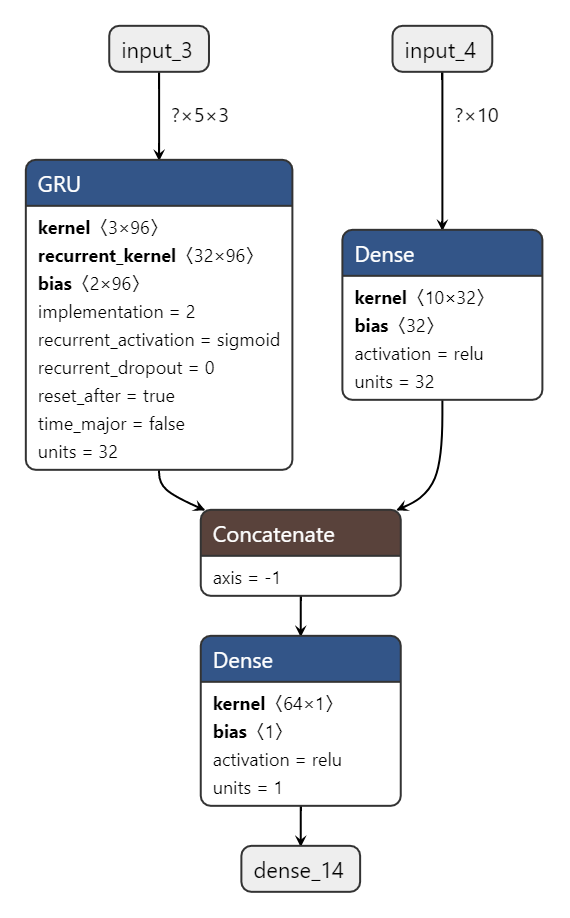
\includegraphics[width=0.7\textwidth]{./Figuras/resultados/case1_rnn_exo_1.png}
                \caption{Model Topology RNN\_EXO\_1.} \label{fig:case1_rnn_exo_1} }
            \end{figure}
        %dropout
        \subsubsection{Endogenous model GRU RNN\_ENDO\_2, best result in the first phase}
           This model was obtained through a second reconfiguration of the first GRU model, RNN\_ENDO\_1 detailed in the figure \ref{fig:case1_rnn_endo1} with the increase in unit depth of this previous model, in regressive format of 16 units in the first layer, 8 units in the second and 4 units in the third, and with the inclusion of the dropout resource based on the topic  \ref{sec:drop_fund}, the final topology is observed in figure \ref{fig:case1_rnn_endo2}. This model produced the best results in the first experimental phase, detailed in figure \ref{fig:case1_rnn_endo2_test_dates} in the next section.
            \begin{figure}[H]
              \center{
                  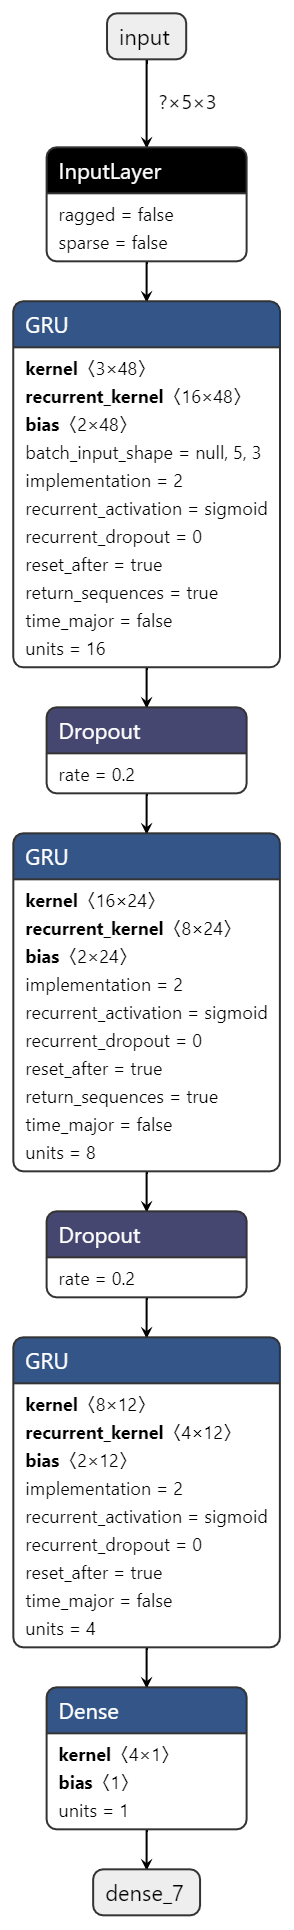
\includegraphics[width=0.24\textwidth]{./Figuras/resultados/case1_rnn_endo2.png}
                  \caption{Model Topology RNN\_ENDO\_2.} 
                  \label{fig:case1_rnn_endo2} 
              }
            \end{figure}
        
    \subsection{Main differences of results between the experimental phases}
        \paragraph{Differences between the best models}
        For the experiments of the 1st phase, the model that produced the smallest RMSE in the set of tests with advantage in all the other metrics was the endogenous model RNN\_ENDO\_2, with some prediction anomalies, as observed in figure \ref{fig:case1_rnn_endo2_test_dates}.
        \begin{figure}[H]
          \center{
            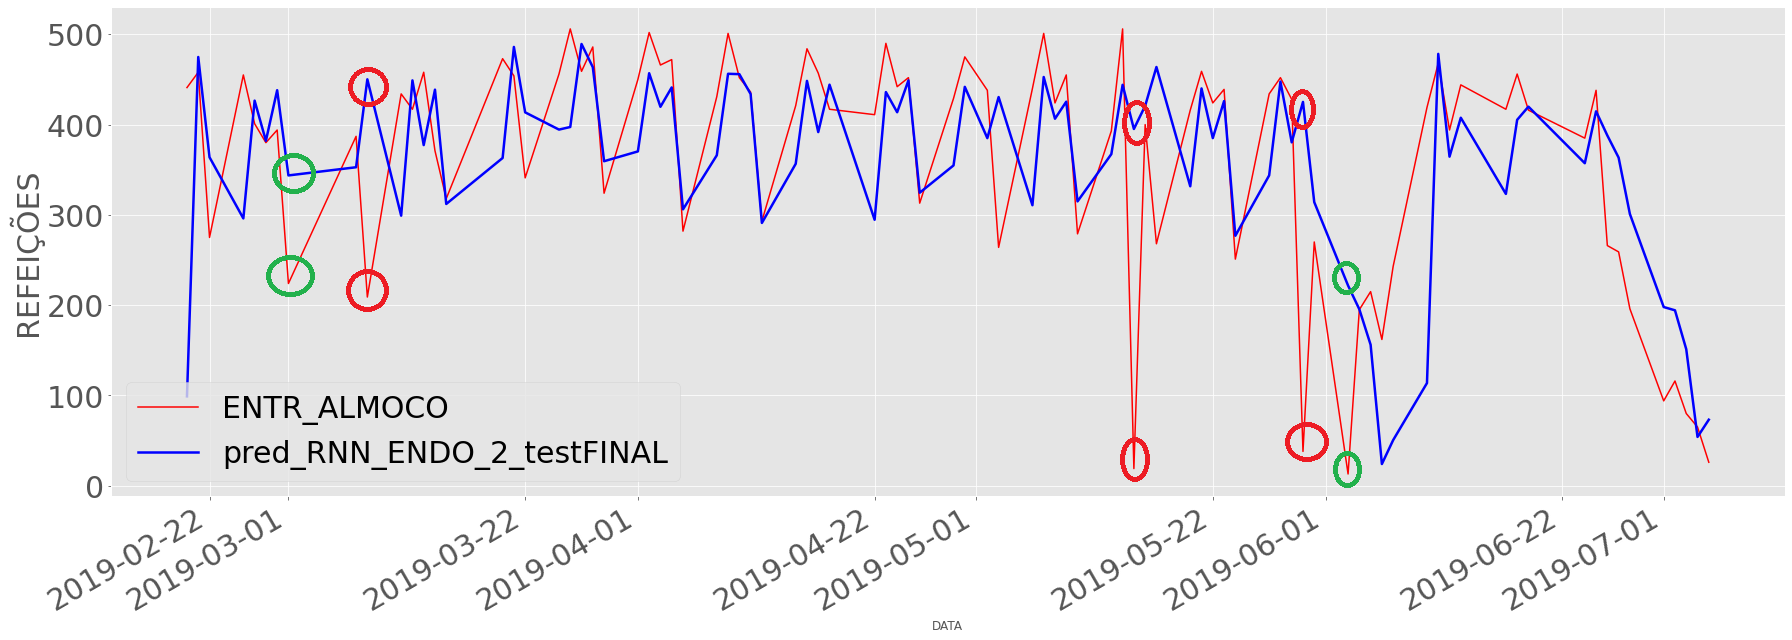
\includegraphics[width=1.0\textwidth]{./Figuras/resultados/case1_rnn_endo2_test_dates.png}
          \caption{Analysis of predictive anomalies of RNN\_ENDO\_2} \label{fig:case1_rnn_endo2_test_dates} }
        \end{figure}
        %dropout
        The green outliers represent predictions that corresponded to an upward or downward trend in consumption but with discrepant errors, and the red outliers represent predictions with an inverse trend in consumption.
        The justifications for the prediction within the trend, are found in the table \ref{table:rnn_endo_2_green}, denoting special dates that could not match the learning process of the model.
            \begin{table}[!ht]
                \centering
                \caption{Model prediction errors RNN\_ENDO\_2 in the 1st phase}
                \label{table:rnn_endo_2_green}
                \rowcolors{2}{gray!25}{white}
                 \begin{tabular}{|c|c|c|}
                 \rowcolor{gray!50}
                 \hline 
                Date & Consumption & Justification\\ \hline    
                03/01/2019 (Friday)    & 224 & Friday pre-carnival\\
                06/03/2019 (Monday)  &  13 & Monday after the student paralyzation\\ \hline 
                \end{tabular} 
            \end{table}
            
        The justifications for forecasts where the model followed the opposite trend to the consumption also corresponded to the special dates, conferred in table \ref{table:rnn_endo_2_red}.
            \begin{table}[!ht]
                \caption{Anomalies of model predictions RNN\_ENDO\_2  in the 1st phase}
                \label{table:rnn_endo_2_red}
                \rowcolors{2}{gray!25}{white}
                 \begin{tabular}{c|c|c}
                 \rowcolor{gray!50}
                 \hline
                Date & Consumption & Justification \\
                03/08/2019 (Friday)   & 209 &Friday after carnival\\
                05/15/2019 (Wednesday)   & 19  & Student paralyzation in Afonso Pena Square\\
                30/05/2019 (Thursday)   &  38  & Student paralyzation in Afonso Pena Square\\
                \hline 
                \end{tabular} 
            \end{table}
        
        In the metrics of this model, it is observed in table \ref{table:rnn_endo_2_test} that the total of positive errors, corresponded to a discard of approximately 3479 meals and the average quadratic error of forecast was approximately 108 meals.
            \begin{table}[!ht]
                \centering
                \rowcolors{2}{gray!25}{white}
                \caption{Metrics from the best model:  RNN\_ENDO\_2 }
                \label{table:rnn_endo_2_test}
                \begin{tabular}{c|c}
                \rowcolor{gray!50}
                \hline
                Best model: &   RNN\_ENDO\_2: \\ \hline
                Total\_Consumed & 31962 \\ 
                Total\_Foreseen & 31465,61133 \\
                Error\_Total\_Forecast & -496,3886719 \\
                Percentage\_Error\_Total & -1,5530\% \\\
               Correlation & 0,595439895 \\
                P-value & 9,42215E-10    \\
                RMSE &  108,0663015\\
                Sum of negative errors. & 2982,567947 \\
                Sum of positive errors. & 3478,957266\\
                ERROR\_ABS\_MEDIAN & 46,70721436 \\ 
                ERROR\_ABSOLUTE\_AVERAGE\_PERCENTUAL & 74,93539002 \\ 
                \hline
                \end{tabular}
            \end{table}
        
        Meanwhile, in the second phase, all the models obtained improvements in the training error over the validation set, and the model with the best predictions of the work was obtained, the mixed model  \textbf{RNN\_EXO\_1} detailed in its own section to follow.
        It is important to note that the 2 phases have produced the best models of different classes, the first with a model that uses only endogenous data, and that includes a validation and test set with a range of only 1 semester, and the second with a model that uses temporal and discrete data and that uses a validation and test set with a range of 1 year.
        This denotes that better results were achieved without any change in parameters and hyper-parameters in the models, changing only the temporal organization of the data sets.
        
        During the testing of all models, only the first semester contemplated special dates where these models produced forecast anomalies, illustrated as an example in figure \ref{fig:case1_rnn_endo2_test_dates}.

\section{Results with the best model, RNN\_EXO\_1}
%\TODO{Nessa seção apresente os resultados do melhor modelo. Se quiser, pode dividir em subseções}
     This model, represented in the figure  \ref{fig:case1_rnn_exo_1} obtained the best results of all this work, when it was training in the second experimental phase.
    It is noticeable its improvement of results with a single change in the organization of the data sets between the experimental phases.
    
    \subsection{Comparison of training between the two phases}
   
     It is observed that this model produced a slower overfitting in the first phase, illustrated in the figure \ref{fig:case1_rnn_exo_1_train} ompared to the training of the second phase demonstrating a convergence to a fast and sharp overfitting from season 100 onwards, bringing better results with the early stopping of training, illustrated in the figure \ref{fig:case2_rnn_exo1_train}. The difference of the RMSE metric values between these 2 trainings, producing a better result in the second phase, of RMSE = 109.97 compared to the result of the first phase of RMSE = 132.94.
     

        \begin{figure}[H]
        \center{                    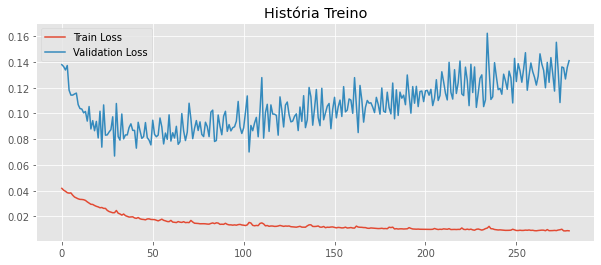
\includegraphics[width=\textwidth]{./Figuras/resultados/case1_rnn_exo_1_train.png}
        \caption{Model training RNN\_EXO\_1  in the 1st phase, RMSE = 132.94} \label{fig:case1_rnn_exo_1_train} }
        \end{figure}

     

    
        \begin{figure}[H]
          \center{
            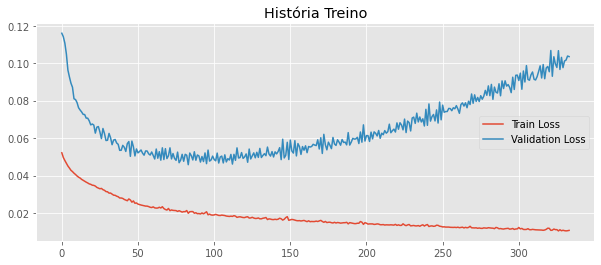
\includegraphics[width=\textwidth]{./Figuras/resultados/case2/case2_rnn_exo1_train.png}
          \caption{Model training graph RNN\_EXO\_1 in second phase, RMSE = 109.97} \label{fig:case2_rnn_exo1_train} }
        \end{figure}
    

    \subsection{Comparative test of the model in the first semester between the two phases}
    
        As this model trained in the second phase obtained the best results of the work, the metrics for the model testing within the domain of the first semester of 2019 were recalculated to make an equivalent comparison with its version trained and tested also in the first semester of 2019 in the first phase.
        
        The table \ref{table:case1_rnn_exo_1} shows that the RMSE testing model trained in the first phase performed less well than the RMSE trained in the second phase according to the table \ref{table:case2_rnn_exo_2_incase1}. The RMSE being smaller in the training of this model in the second phase brings an improvement in all other metrics compared to its training in the first phase.
        The sum of the positive prediction errors was also lower in the second phase, which impacts less on meal disposal.
        The RMSE of this model tested in the first phase and reaching RMSE = 106.208 also did better than the best model of the first phase, the RNN\_ENDO\_2 which reached RMSE = 108.06.
        
        
        
        
        \begin{table}[!ht]
            \centering
            \caption{RNN\_EXO\_1 TRAINED IN PHASE 1,TEST FIRST SEMESTER 2019}
            \label{table:case1_rnn_exo_1}
            \rowcolors{2}{gray!25}{white}
                \begin{tabular}{c|c}
                \rowcolor{gray!50}
                \hline
            \multicolumn{2}{c}{RNN\_EXO\_1 TRAINED IN PHASE 1,TEST FIRST SEMESTER 2019} \\
            \hline
            RMSE & 124.49\\
            TOTAL MEALS CONSUMED & 31962 \\
            TOTAL OF PROJECTED MEALS & 28728.816  \\
            FORECAST ERROR & -3233.1839 \\
            PERCENTAGE ERROR& -10.11\%  \\
            CORRELATION (r) & 0.41 \\ 
            P-value & 6.59e-05\\ 
            R2 & 0.16\\
            SUM OF POSITIVE ERRORS & 2709.17\\
            SUM OF NEGATIVE ERRORS & 5942.35\\
            MEDIAN ABSOLUTE ERROR & 85.59\\
            ABSOLUTE ERROR AVERAGE PERCENTAGE & 90.98\% \\ \hline \end{tabular} \end{table}
            
      
      
            \begin{table}[!ht]
            \centering
            \caption{RNN\_EXO\_1 TRAINED IN PHASE 2,TEST FIRST SEMESTER 2019}
            \label{table:case2_rnn_exo_2_incase1}
            \rowcolors{2}{gray!25}{white}
                \begin{tabular}{c|c}
                \rowcolor{gray!50}
                \hline
                \multicolumn{2}{c}{RNN\_EXO\_1 TRAINED IN PHASE 2,TEST FIRST SEMESTER 2019}\\ \hline
                RMSE & 106.2080\\
                TOTAL MEALS CONSUMED & 31962\\
                TOTAL OF PROJECTED MEALS & 32170.24\\
                FORECAST ERROR & 208.2460 \\
                PERCENTAGE ERROR & 0.6515\%  \\
                CORRELATION (r)& 0.59 \\
                P-value (p) & 1.4143e-09\\
                R2 & 0.3485\\
                SUM OF POSITIVE ERRORS & 3454.8698\\
                SUM OF NEGATIVE ERRORS & 3246.6228\\
                MEDIAN ABSOLUTE ERROR & 59.5414\\
                ABSOLUTE ERROR AVERAGE PERCENTAGE & 83.2671\% \\ \hline
            \end{tabular}
            \end{table}
                
            
            
        The scatter plot of the trained model in the first phase as shown in figure \ref{fig:case1_rnn_exo_1_test_scatter} also came out worse, farther from the upper right edge of the plot, than the scatter plot of the trained model in the second phase as shown in figure  \ref{fig:case2_rnn_exo2_test_incase1_Figura}.
        
                \begin{figure}[H]
                      \center{                    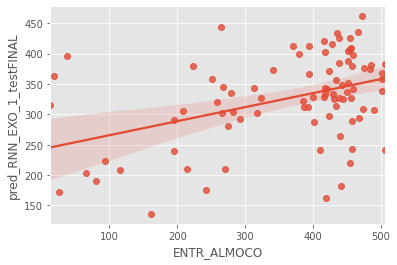
\includegraphics[width=\textwidth]{./Figuras/resultados/case1_rnn_exo_1_test_scatter.png}
                        \caption{Model test dispersion graph RNN\_EXO\_1, first phase} \label{fig:case1_rnn_exo_1_test_scatter} }
                        \end{figure}        
        


     \begin{figure}[H]
              \center{
                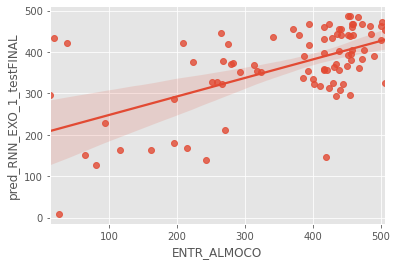
\includegraphics[width=\textwidth]{./Figuras/resultados/case2/case2_rnn_exo2_test_incase1_scatter.png}
              \caption{Test scatter plot of the first semester, RNN\_EXO\_1 trained in the second phase.} \label{fig:case2_rnn_exo2_test_incase1_Figura} }
                \end{figure}        In conclusion, when comparing the prediction graphs, the  RNN\_EXO\_1 model trained in the first phase produced worse predictions, and did not learn the weekly seasonality of consumption, as can be seen in figure  \ref{fig:case1_rnn_exo_1_test}, it is also possible to notice in table  \ref{table:case1_rnn_exo_1}, that the correlation between the predicted values and actual consumption, as well as the value  $R^2$ was lower compared to the metrics of the model trained in the second phase, and that this model trained in the second phase learned better the weekly and monthly seasonality of consumption as can be seen in the figure \ref{fig:case2_rnn_exo2_test_incase1}.
      
           
                  \begin{figure}[H]
                      \center{                    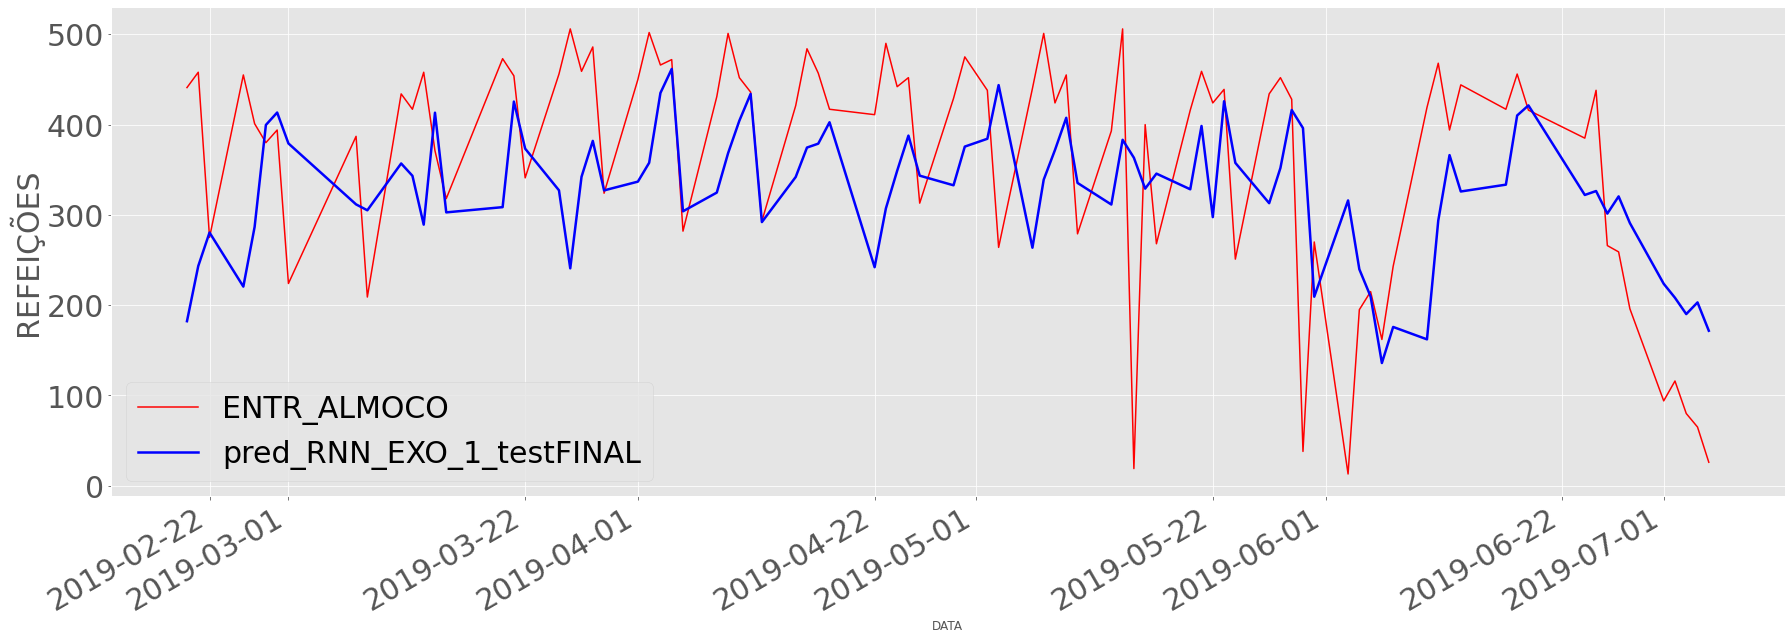
\includegraphics[width=\textwidth]{./Figuras/resultados/case1_rnn_exo_1_test.png}
                      \caption{Model Test  RNN\_EXO\_1, 1 Phase} 
                      \label{fig:case1_rnn_exo_1_test} }
                    \end{figure} 

   

            
            
      
           
           
            \begin{figure}[H]
              \center{
                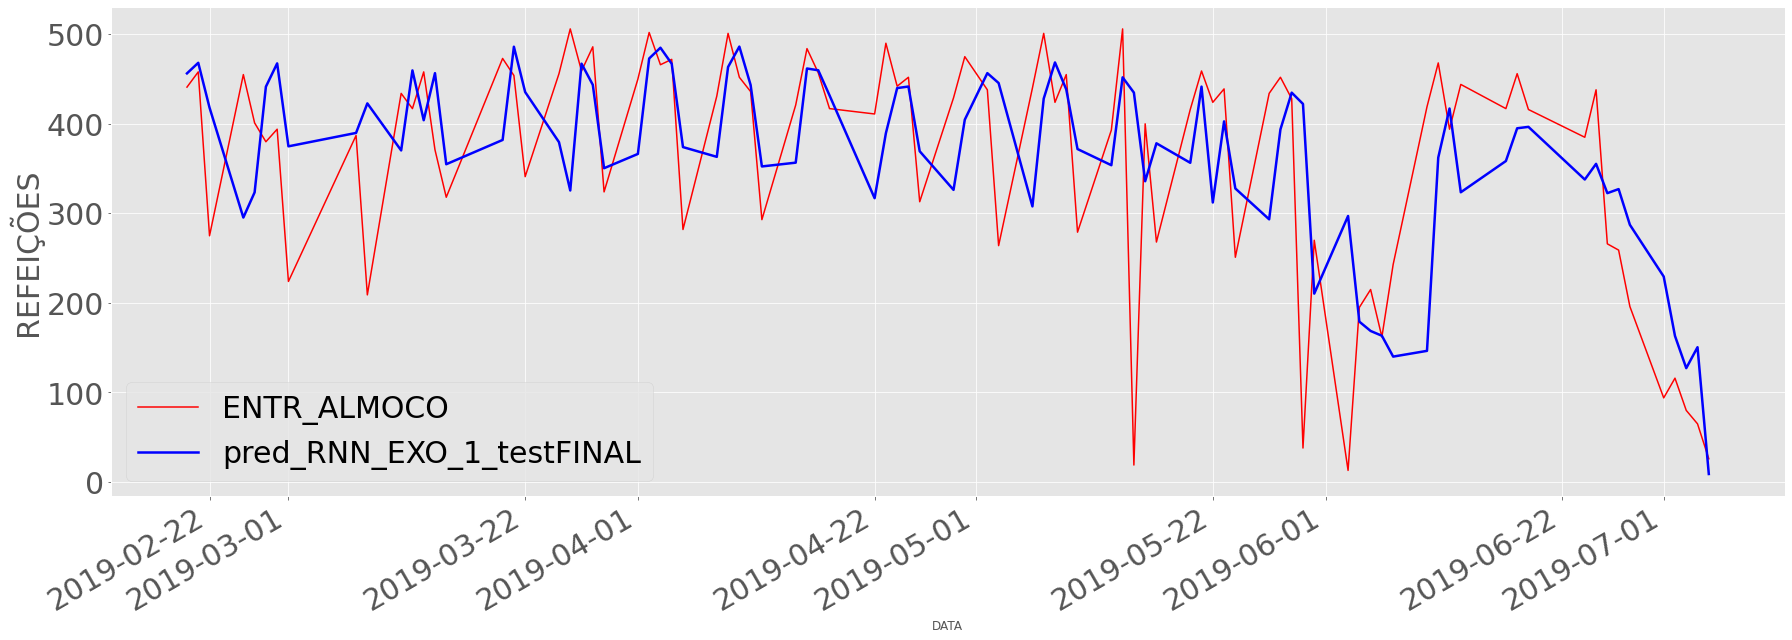
\includegraphics[width=\textwidth]{./Figuras/resultados/case2/case2_rnn_exo2_test_incase1.png}
              \caption{Test of the first semester of RNN\_EXO\_1 trained in the second phase.} \label{fig:case2_rnn_exo2_test_incase1} }
            \end{figure}
           
           
           
                
                
                
    \subsection{Final test of the  RNN\_EXO\_1 model for the ICT-Unifesp R.U predictions}
    
     The final test of RNN\_EXO\_1 produced the best results with its training in the second phase and being tested for the entire year 2019. The RMSE observed in table  \ref{table:case2_rnn_exo_2_2019} was notoriously inferior to all the models trained and tested in all the research.
     
      
        \begin{table}[!h]
            \centering
            \caption{RNN\_EXO\_1 TRAINED IN THE 2ND PHASE, TEST YEAR 2019}
            \label{table:case2_rnn_exo_2_2019}
            \rowcolors{2}{gray!25}{white}
                \begin{tabular}{c|c}
                \rowcolor{gray!50}
                \hline
                \multicolumn{2}{c}{RNN\_EXO\_1 TRAINED IN THE 2ND PHASE, TEST YEAR 2019}\\ \hline
                RMSE & 99.36\\
                TOTAL MEALS CONSUMED & 58653 \\
                TOTAL OF PROJECTED MEALS & 62048.04\\
                FORECAST ERROR & 3395.04 \\
                PERCENTAGE ERROR  & 5.78\%  \\
                CORRELATION (r)& 0.67 \\
                P-value (p) & 3.29e-25\\
                R2 & 0.45\\
                SUM OF POSITIVE ERRORS  & 8163.18\\
                SUM OF NEGATIVE ERRORS  & 4768.13\\
                MEDIAN ABSOLUTE ERROR  & 55.23\\
                ABSOLUTE ERROR AVERAGE PERCENTAGE & 83.2671\% \\ \hline
            \end{tabular}
            \end{table}

    \newpage
     The disposal of meals was obtained by the sum of the positive errors reached the value of 4768 meals.
     In the figure\ref{fig:case2_rnn_exo1_test} it is possible to notice that the model learned well the monthly and weekly seasonality of the consumption, but obtained a discrepant error for the first predicted value of the second semester, the error was justifiable because its training set contemplates only 1 year with 1 alternation of semester making impossible a better learning about this behavior.
     The scatter plot illustrated in the figure \ref{fig:case2_rnn_exo1_test_scatter} lso demonstrates a good linear regression over the predicted values of the model and the actual consumption value, approaching the identity function of an ideal forecast.
     
            %%% RNN_EXO_1
        \begin{figure}[H]
          \center{
            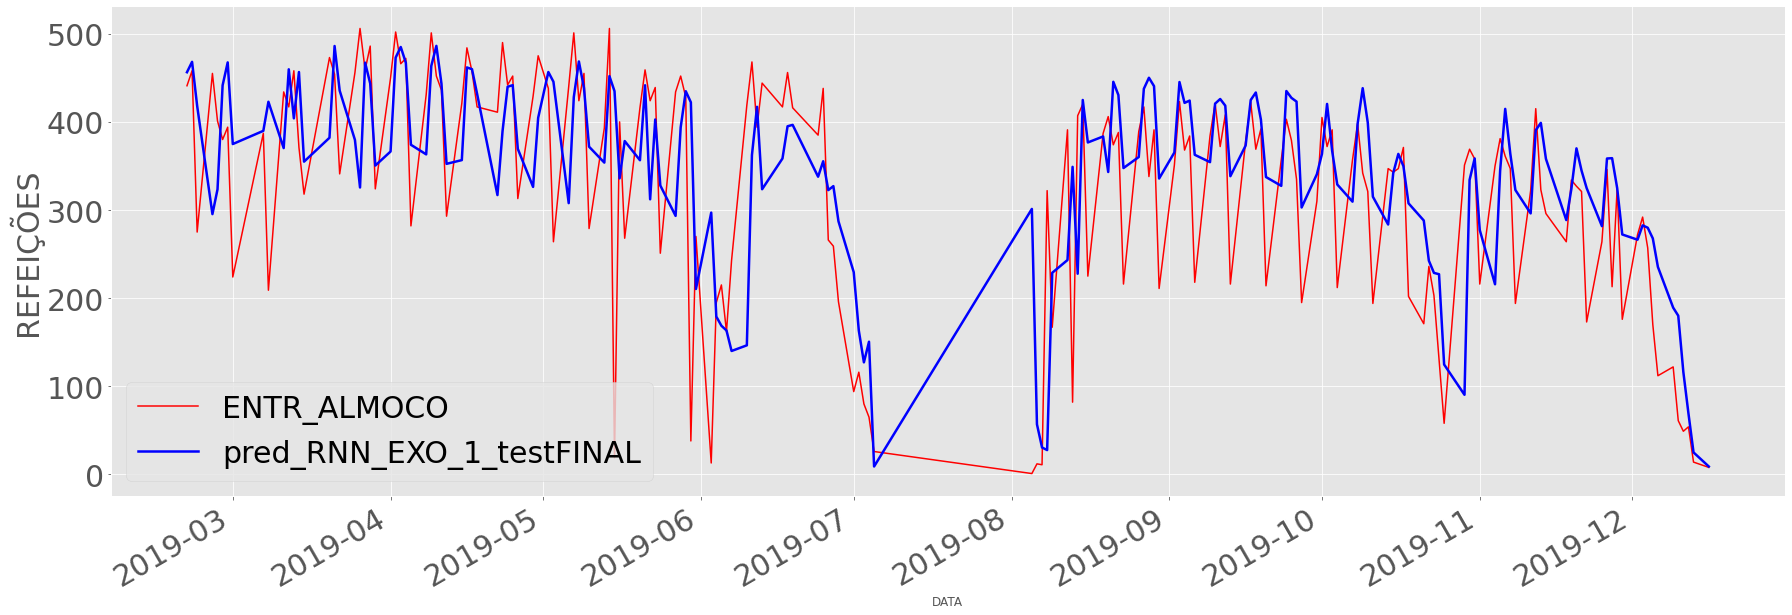
\includegraphics[width=\textwidth]{./Figuras/resultados/case2/case2_rnn_exo1_test.png}
          \caption{Final Test Graph of the Model RNN\_EXO\_1.} \label{fig:case2_rnn_exo1_test} }
        \end{figure}
       
       
        \begin{figure}[H]
          \center{
            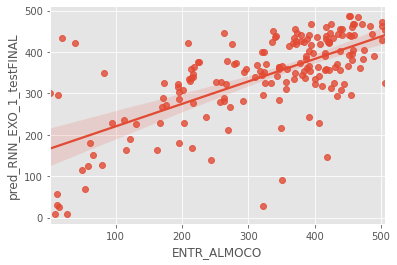
\includegraphics[width=\textwidth]{./Figuras/resultados/case2/case2_rnn_exo1_test_scatter.png}
          \caption{Model Dispersion Graph  RNN\_EXO\_1.} \label{fig:case2_rnn_exo1_test_scatter} }
        \end{figure}
        
        Results obtained by the other tested methods are available in the \ref{chapter:outros}.
       
